% Title page, abstract, contents, nomenclature

\begin{titlepage}
  \centering
  \vspace*{0.4in}
  {\LARGE\bfseries Design and Testing of an Autonomous Tracked Robot for Monarch of the Hill \par}
  \vspace{0.25in}
  {\large Monarch of the Hill, AME 101, Fall 2026\par}
  \vspace{0.3in}
  {\normalsize Team 2: Gabriel Oliveri, Charlie Haldeman, Efe Altinkaya, Ashley Valdez\par}
  \vspace{0.08in}
  {\normalsize University of Southern California\par}
  \vspace{0.4in}
  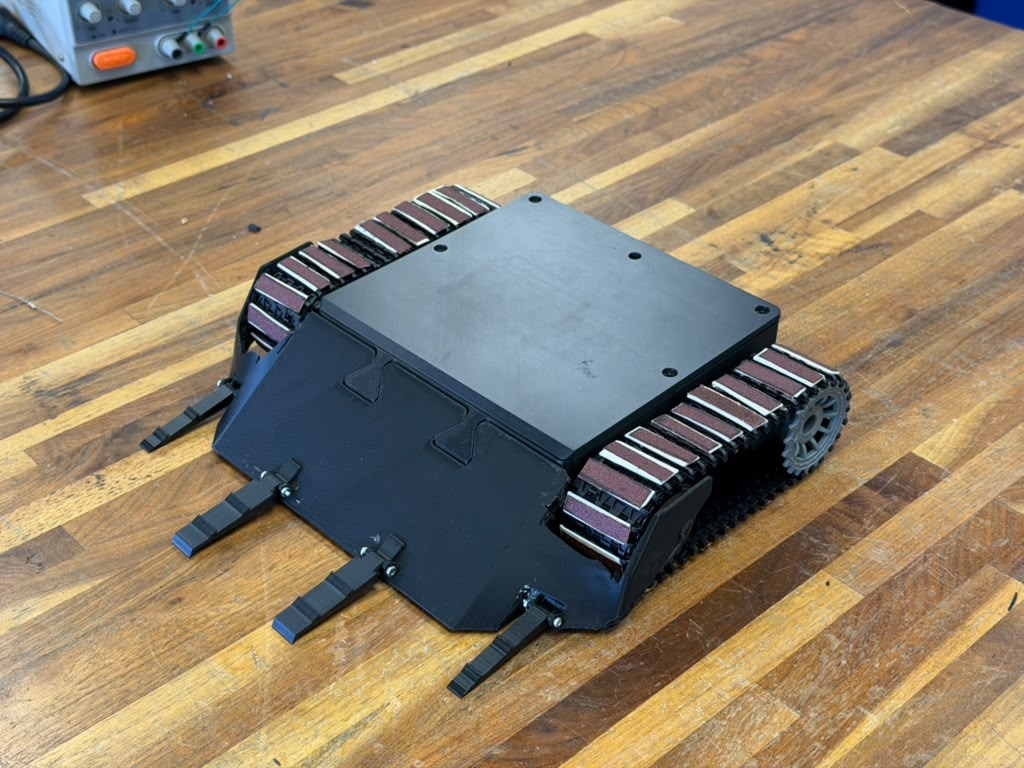
\includegraphics[width=0.62\textwidth]{title_robot.jpg}\par
  \vfill
  \begin{tabular}{@{}lr@{}}
    \toprule
    \textbf{Category} & \textbf{Score} \\
    \midrule
    Organization    & /20 \\
    Documentation   & /35 \\
    Testing         & /25 \\
    Lessons learned & /20 \\
    \midrule
    Total           & /100 \\
    \bottomrule
  \end{tabular}\par
  \vspace*{0.1in}
\end{titlepage}

\setcounter{page}{2}

\section*{Abstract}
\addcontentsline{toc}{section}{Abstract}
We designed and built an autonomous tracked robot for the AME 101 Monarch of the Hill contest. Two robots start at the bottoms of opposite \ang{33.4} ramps, and after \qty{30}{s} the robot whose farthest point is closest to the center of the shared summit wins. Our strategy was to reach the summit first and never depend on a pushing match: a low wedge with forks at the front lets an arriving opponent drive up and over us, and running along a side wall replaces steering. The robot uses two \qty{25}{mm}, \qty{280}{\rpm} gearmotors on the stock sprockets with sandpaper on the tracks, a SparkFun TB6612FNG motor driver and a Particle Photon~2 controller. It tracks its pitch with a complementary filter that combines gyro and accelerometer readings, because the accelerometer alone misreads pitch whenever the robot speeds up or slows down. It climbs the \qty{1.52}{m} ramp in about \qty{3.3}{s} (timed by stopwatch) and weighs \qty{1.000}{kg} against the \qty{1}{kg} limit. We won the contest with a 5--1 record. Our one loss, in the final round, came from run-to-run variation in the timed climb: the robot stopped short on the mesa, and the opponent's farthest point ended up closer to the center. Our main lesson is to triage hard: dropping complex ideas early left enough time to test the robot and its software.

\vspace{0.5\baselineskip}
{\setlength{\parskip}{0pt}\setcounter{tocdepth}{1}\tableofcontents}

\clearpage
\section*{Nomenclature}
\addcontentsline{toc}{section}{Nomenclature}

{\small\renewcommand{\arraystretch}{0.84}
\begin{tabularx}{\textwidth}{@{}l L l@{}}
  \toprule
  \textbf{Symbol} & \textbf{Meaning} & \textbf{Units} \\
  \midrule
  $a$ & acceleration along the ramp & \unit{m/s^2} \\
  $\bm{a}_\mathrm{m}$ & acceleration vector measured by the accelerometer & \unit{m/s^2} \\
  $c$ & distance from the neutral axis to the outermost fiber & \unit{mm} \\
  $F$ & traction force from both tracks & \unit{N} \\
  $F(v)$, $F_\mathrm{stall}$ & drive force from both motors at speed $v$; at stall & \unit{N} \\
  $F_f$ & static friction force between the tracks and the ramp & \unit{N} \\
  $F_\mathrm{att}$, $F_\mathrm{def}$ & largest force an attacker on the ramp can push with; largest force a defender on the mesa can resist with & \unit{N} \\
  $G$ & gear ratio & -- \\
  $g$ & gravitational acceleration, 9.81 & \unit{m/s^2} \\
  $I$ & second moment of area of a section; current drawn from the pack (Eq.~\eqref{eq:vterm}) & \unit{mm^4}; \unit{A} \\
  $I_\mathrm{m}$, $I_\mathrm{stall}$, $I_\mathrm{stall,max}$ & motor current; at stall; largest stall current the pack allows & \unit{A} \\
  $k_\mathrm{t}$ & motor torque constant & \unit{N.m/A} \\
  $k_r$ & resistance factor: total resistance to climbing as a multiple of $m g \sin\ang{33.4}$ & -- \\
  $M$ & bending moment & \unit{N.m} \\
  $m$ & robot mass & \unit{kg} \\
  $N$ & normal force & \unit{N} \\
  $P_\mathrm{max}$ & peak mechanical power per motor & \unit{W} \\
  $R_\mathrm{w}$ & motor winding resistance & \unit{\ohm} \\
  $R_\mathrm{int}$ & pack internal resistance & \unit{\ohm} \\
  $r$ & sprocket rolling radius & \unit{m} \\
  $T$, $T_\mathrm{max}$ & total tension of the tread on the sprocket; tension at which the coupler fails & \unit{N} \\
  $T(G)$ & climb time with gear ratio $G$ & \unit{s} \\
  $T_c$ & filter time constant & \unit{s} \\
  $t_0$ & time constant of the approach to $v_t$ & \unit{s} \\
  $\Delta t$ & filter update interval & \unit{s} \\
  $\hat{\bm{u}}$ & estimated direction of gravity in the sensor frame & -- \\
  $\hat{\bm{z}}$ & the robot's up direction in the sensor frame & -- \\
  $V$ & pack voltage & \unit{V} \\
  $V_\mathrm{term}$ & pack terminal voltage under load & \unit{V} \\
  $\Delta V_\mathrm{sag}$ & drop in pack voltage with both motors at stall & \unit{V} \\
  $v$, $v_0$, $v_t$ & speed along the ramp; no-load; steady climbing & \unit{m/s} \\
  $W$ & total resistance to climbing, $k_r m g \sin\ang{33.4}$ & \unit{N} \\
  $\mathcal{E}$ & pack open-circuit voltage & \unit{V} \\
  $\ell$ & lever arm from the bottom of the motor bore to the tread line & \unit{mm} \\
  \midrule
  \multicolumn{3}{@{}l}{\textit{Greek symbols}} \\
  $\eta_\mathrm{g}$ & gearbox efficiency & -- \\
  $\theta$, $\theta_\mathrm{apparent}$ & robot pitch; pitch implied by the accelerometer alone & \unit{\degree} \\
  $\mu_s$ & static friction coefficient, tracks on the ramp surface & -- \\
  $\sigma$, $\sigma_\mathrm{allow}$ & bending stress; failure stress of the print & \unit{MPa} \\
  $\tau_\mathrm{m}$ & torque of one motor & \unit{N.m} \\
  $\bm{\omega}$ & gyro angular rate & \unit{rad/s} \\
  $\omega_\mathrm{m}$ & motor shaft speed & \unit{rad/s} \\
  \bottomrule
\end{tabularx}
}

\clearpage
